% This is "sig-alternate.tex" V1.9 April 2009
% This file should be compiled with V2.4 of "sig-alternate.cls" April 2009
%
% This example file demonstrates the use of the 'sig-alternate.cls'
% V2.4 LaTeX2e document class file. It is for those submitting
% articles to ACM Conference Proceedings WHO DO NOT WISH TO
% STRICTLY ADHERE TO THE SIGS (PUBS-BOARD-ENDORSED) STYLE.
% The 'sig-alternate.cls' file will produce a similar-looking,
% albeit, 'tighter' paper resulting in, invariably, fewer pages.
%
% ----------------------------------------------------------------------------------------------------------------
% This .tex file (and associated .cls V2.4) produces:
%       1) The Permission Statement
%       2) The Conference (location) Info information
%       3) The Copyright Line with ACM data
%       4) NO page numbers
%
% as against the acm_proc_article-sp.cls file which
% DOES NOT produce 1) thru' 3) above.
%
% Using 'sig-alternate.cls' you have control, however, from within
% the source .tex file, over both the CopyrightYear
% (defaulted to 200X) and the ACM Copyright Data
% (defaulted to X-XXXXX-XX-X/XX/XX).
% e.g.
% \CopyrightYear{2007} will cause 2007 to appear in the copyright line.
% \crdata{0-12345-67-8/90/12} will cause 0-12345-67-8/90/12 to appear in the copyright line.
%
% ---------------------------------------------------------------------------------------------------------------
% This .tex source is an example which *does* use
% the .bib file (from which the .bbl file % is produced).
% REMEMBER HOWEVER: After having produced the .bbl file,
% and prior to final submission, you *NEED* to 'insert'
% your .bbl file into your source .tex file so as to provide
% ONE 'self-contained' source file.
%
% ================= IF YOU HAVE QUESTIONS =======================
% Questions regarding the SIGS styles, SIGS policies and
% procedures, Conferences etc. should be sent to
% Adrienne Griscti (griscti@acm.org)
%
% Technical questions _only_ to
% Gerald Murray (murray@hq.acm.org)
% ===============================================================
%
% For tracking purposes - this is V1.9 - April 2009

\documentclass{sig-alternate-05-2015}
  \pdfpagewidth=8.5truein
  \pdfpageheight=11truein

\usepackage{verbatim}
\usepackage{graphicx}
\usepackage{subcaption}
\usepackage{hyperref}
\usepackage{listings}
\usepackage{courier}
\usepackage{epstopdf}

% \lstset{language=[Sharp]C}
\lstset{numbers=left,xleftmargin=3em,numberstyle=\footnotesize\ttfamily,captionpos=b}
\lstset{basicstyle=\footnotesize\ttfamily}

\begin{document}
\setcopyright{acmlicensed}
%
% --- Author Metadata here ---
% \conferenceinfo{SAC'15}{April 13-17, 2015, Salamanca, Spain.}
% \CopyrightYear{2015} % Allows default copyright year (2002) to be over-ridden - IF NEED BE.
% \crdata{978-1-4503-3196-8/15/04}  % Allows default copyright data (X-XXXXX-XX-X/XX/XX) to be over-ridden.
% --- End of Author Metadata ---

\title{On Development of Static Analysis Tools for String-Embedded Languages}
% \subtitle{[Extended Abstract]
% \titlenote{A full version of this paper is available as
% \textit{Author's Guide to Preparing ACM SIG Proceedings Using
% \LaTeX$2_\epsilon$\ and BibTeX} at
% \texttt{www.acm.org/eaddress.htm}}}
%
% You need the command \numberofauthors to handle the 'placement
% and alignment' of the authors beneath the title.
%
% For aesthetic reasons, we recommend 'three authors at a time'
% i.e. three 'name/affiliation blocks' be placed beneath the title.
%
% NOTE: You are NOT restricted in how many 'rows' of
% "name/affiliations" may appear. We just ask that you restrict
% the number of 'columns' to three.
%
% Because of the available 'opening page real-estate'
% we ask you to refrain from putting more than six authors
% (two rows with three columns) beneath the article title.
% More than six makes the first-page appear very cluttered indeed.
%
% Use the \alignauthor commands to handle the names
% and affiliations for an 'aesthetic maximum' of six authors.
% Add names, affiliations, addresses for
% the seventh etc. author(s) as the argument for the
% \additionalauthors command.
% These 'additional authors' will be output/set for you
% without further effort on your part as the last section in
% the body of your article BEFORE References or any Appendices.

\numberofauthors{3} %  in this sample file, there are a *total*
% of EIGHT authors. SIX appear on the 'first-page' (for formatting
% reasons) and the remaining two appear in the \additionalauthors section.
%
\author{
% You can go ahead and credit any number of authors here,
% e.g. one 'row of three' or two rows (consisting of one row of three
% and a second row of one, two or three).
%
% The command \alignauthor (no curly braces needed) should
% precede each author name, affiliation/snail-mail address and
% e-mail address. Additionally, tag each line of
% affiliation/address with \affaddr, and tag the
% e-mail address with \email.
%
% 1st. author
% 1st. author
\alignauthor Marat Khabibullin\\
       \affaddr{St. Petersburg Academic University}\\
       \affaddr{194021, Khlopina Str 8/3}\\
       \affaddr{St. Petersburg, Russia}\\
       \email{maratx387@gmail.com}
% 2nd. author       
\alignauthor Andrei Ivanov\\ 
       \affaddr{St. Petersburg State University}\\
       \affaddr{198504, Universitetsky prospekt 28}\\
       \affaddr{Peterhof, St. Petersburg, Russia}\\
       \email{ivanovandrew2004@gmail.com}
\and
% 3rd. author
\alignauthor Semyon Grigorev\\ 
       \affaddr{St. Petersburg State University}\\
       \affaddr{198504, Universitetsky prospekt 28}\\
       \affaddr{Peterhof, St. Petersburg, Russia}\\
       \email{rsdpisuy@gmail.com}
}
% There's nothing stopping you putting the seventh, eighth, etc.
% author on the opening page (as the 'third row') but we ask,
% for aesthetic reasons that you place these 'additional authors'
% in the \additional authors block, viz.
% \additionalauthors{Additional authors: John Smith (The
% Th{\o}rv{\"a}ld Group, email: {\texttt{jsmith@affiliation.org}})
% and Julius P.~Kumquat (The Kumquat Consortium, email:
% {\texttt{jpkumquat@consortium.net}}).}
\date{27 July 2015}
% Just remember to make sure that the TOTAL number of authors
% is the number that will appear on the first page PLUS the
% number that will appear in the \additionalauthors section.

\maketitle

\begin{abstract}

Some programs can produce string expressions with embedded code in other programming languages while running. This embedded code should be syntactically correct as it is typically executed by some subsystem. A program in Java language that builds and sends SQL queries to the database it works with can be considered as an example. In such scenarios, languages like SQL are called string-embedded and ones like Java -- host languages.

In spite of the fact such an approach of programs building is being replaced by alternative ones, for example by ORM and LINQ, string-embedding is still used in practice. Development and reengineering of the programs with string-embedded languages is complicated because the IDE and similar tools process the code embedded in strings as host language string literals and cannot provide the functionality to work with this code. To facilitate the development process, string-embedded code highlighting, completion, navigation and static errors checking would be useful. For the purposes of reengineering, embedded code metrics computation would be helpful.

Currently existing tools to string-embedded languages support only operate with one host language and a fixed set of string-embedded ones. Their functionality is often limited. Moreover, it is almost impossible or requires a substantial amount of work to add a support for both new host and string-embedded language. Attempts to extend their functionality often result in the same problem. 

In this paper we present the platform which can be used for relatively fast and easy building of endpoint tools that provide a support for different string-embedded languages inside different host languages. The tools built for T-SQL and arithmetic expressions language embedding in C\# are demonstrated as the examples of how the platform can be used.
\end{abstract}

\begin{CCSXML}
<ccs2012>
    <concept>
        <concept_id>10011007.10010940.10010992.10010998.10011000</concept_id>
        <concept_desc>Software and its engineering~Automated static analysis</concept_desc>
        <concept_significance>500</concept_significance>
    </concept>
    <concept>
        <concept_id>10011007.10011006.10011073</concept_id>
        <concept_desc>Software and its engineering~Software maintenance tools</concept_desc>
        <concept_significance>500</concept_significance>
    </concept>
    <concept>
        <concept_id>10003752.10010124.10010138.10010143</concept_id>
        <concept_desc>Theory of computation~Program analysis</concept_desc>
        <concept_significance>300</concept_significance>
    </concept>
    <concept>
        <concept_id>10003752.10010124.10010138.10010145</concept_id>
        <concept_desc>Theory of computation~Parsing</concept_desc>
        <concept_significance>300</concept_significance>
    </concept>
</ccs2012>
\end{CCSXML}

\ccsdesc[500]{Software and its engineering~Automated static analysis}
\ccsdesc[500]{Software and its engineering~Software maintenance tools}
\ccsdesc[300]{Theory of computation~Program analysis}
\ccsdesc[300]{Theory of computation~Parsing}

\printccsdesc

\keywords{String-embedded language, integrated development environment, IDE, approximation, control flow graph, CFG}

\section{Introduction}
When writing certain kinds of programs on some programming language one frequently needs to construct a code on some other language. The program written on Java, C\# or PHP constructing SQL queries and sending them to the database can be considered as an example. In such a program SQL queries can be constructed as string literals, both by writing the entire query inside the literal or by forming final query dynamically, i.e. by combining parts using string operations (concatenation, replace) and common language constructions (loops, conditional expressions). It is important to note that in the later case the parts are no need to be correct SQL expressions. Other examples of the approach in question include forming JavaScript code inside Java when writing web-applications, building of dynamic SQL queries using Dynamic-SQL, xml-files generation, etc. The language that manipulates strings containing code is called the host language. The language which code is written inside string literals is called string-embedded language.

It is useful to have the ability to perform static analysis on string-embedded languages. On the one hand, such analysis would make it possible to support string-embedded languages in IDEs by making syntax highlighting, static errors checking and other functions, previously only available for host languages, become available for string-embedded ones right inside string literals. On the other hand, programs writing approach under consideration is more and more frequently replaced by more advanced approaches. For example, speaking about embedded SQL such approaches include ORM (object-relational mapping) and LINQ (language integrated query). In spite of this fact, there exist many programs where string-embedded languages are used. These programs are still in use so they need a support and maintenance. In particular reengineering can be performed for them. 

Static analysis can be useful during the reengineering process at least in two ways. The first one is extracting some information about string-embedded code. Examples include estimating embedded program's structural complexity using such metrics as cyclomatic complexity~\cite{cyclomatic:ref}, or, in the case of embedded SQL, estimating tables usage frequency in queries to check the possibility of restructuring the database the embedded program works with. The second way is automated transformation of the embedded code to move from the string embedding approach to alternative ones (for example, to move from string-embedded SQL to LINQ). It is important to note that the possibility of such transformations in general case is questionable even in theory. However, in particular cases such transformations can be performed automatedly.

The problem of string-embedded languages static analysis poses a number of challenges. Firstly, not all string expressions in a program contain embedded code and analyzer must be able to differentiate one expressions from another. Secondly, as it was mentioned before, string expressions can be formed dynamically. Thus, we need to construct them according to the operations they are formed with before we can start the analysis itself. Thirdly, the program in the host language in general case may produce the set of strings with embedded code so the analyzer must be able to build this set and represent it in a way convenient for the following analysis. Finally, the lexical and syntax analysis algorithms that can work not only with a single string but with the set of strings are needed.

Despite the utility of string-embedded languages static analysis, existing tools are mostly intended to support embedded code in IDEs and can hardly be used for reengineering problems solving. Moreover, the majority of the tools work only with specific host and string-embedded languages.

In this paper we present the platform for string-embedded languages support, which is a part of the  YaccConstructor~\cite{YaccConstructor:ref} project. The YaccConstructor is devoted to the experiments in the field of static analysis. The platform under discussion is intended as a basis for endpoint tools, making the process of its creation relatively easy and fast. Endpoint tools can be created for different host and string-embedded languages. The platform is designed to be extensible, so it is able to add different functions based on string-embedded language static analysis (from the syntax highlighting to metrics computation). This paper describes the platform and shows how to create endpoint tools.

\section{Existing tools}

There are several tools that can process dynamically generated expressions. Many of them are oriented to support string-embedded languages in IDE. Such tools implement one of two basic approaches. 
\begin{itemize}
\item{Language inclusion checking. This approach answers the question if the strings generated by a program is included in the reference language described by user. This approach can be used to check expressions correctness, but other kinds of analysis cannot be performed based on the approach under consideration.  }
\item{Approximation of dynamically generated expression set followed by lexical and syntax analysis. By expressions set approximation one means the process of building a subset or a superset of the initial one. In the case of superset building it is called upper approximation. The advantages of the approach in question include flexibility: each step is performed independently, so existing algorithms implementations can be used for each step and can be replaced by other implementations if needed. As a result new tools can be created based on the existing ones.}
\end{itemize}

Below a brief description of currently available tools is given.

\subsection{JSA}
The Java String Analyzer\footnote{Java String Analyzer project site:\url{http://www.brics.dk/JSA/}}~\cite{JSA:ref} is a tool to analyze the flow of strings and string operations in Java programs. JSA checks if the regular approximation of the embedded language is included in the context-free description of the reference language. For every string expression JSA computes a finite-state automaton (FSA). It represents the approximate set of string expression's possible values that may be produced during the program execution. To build the FSA, the context-free grammar is constructed from the program's data-flow graph. This grammar is obtained by replacing every string variable with nonterminal, every string literal with terminal and every string operation with production rule. Then the context-free language the grammar produces is approximated by the regular one. As a result the tool returns the strings that are not in the reference language but that can be produced during the program execution.


\subsection{PHPSA}
PHP string analyzer\footnote{PHP String Analyzer project site:\url{http://www.score.cs.tsukuba.ac.jp/~minamide/phpsa/}}~\cite{PHPSA:ref} is a static program analyzer that supports HTML and XML code embedded in PHP. The approach is based on the ideas used in JSA but to increase the analysis accuracy the context-free approximation is used instead of the regular one.

\subsection{Alvor}

Alvor\footnote{Alvor project site:\url{https://bitbucket.org/plas/alvor}}~\cite{Alvor:ref} is a plugin for Eclipse IDE that is intended for a static validation of SQL expressions embedded into Java code. Alvor performs the interprocedural code analysis, processes conditional statements, concatenation and assignment operations and reports lexical and syntax errors. If more than one error is detected only the first one is reported. The example of such a case is represented in Figure~\ref{alvor_pic}, with typos in lines 16 and 18. Only the typo in the line 16 is indicated by underlining. However, it should be mentioned that the plugin lacks loops and string operations other than concatenation support.

\begin{figure}[h!]
    \begin{center}
        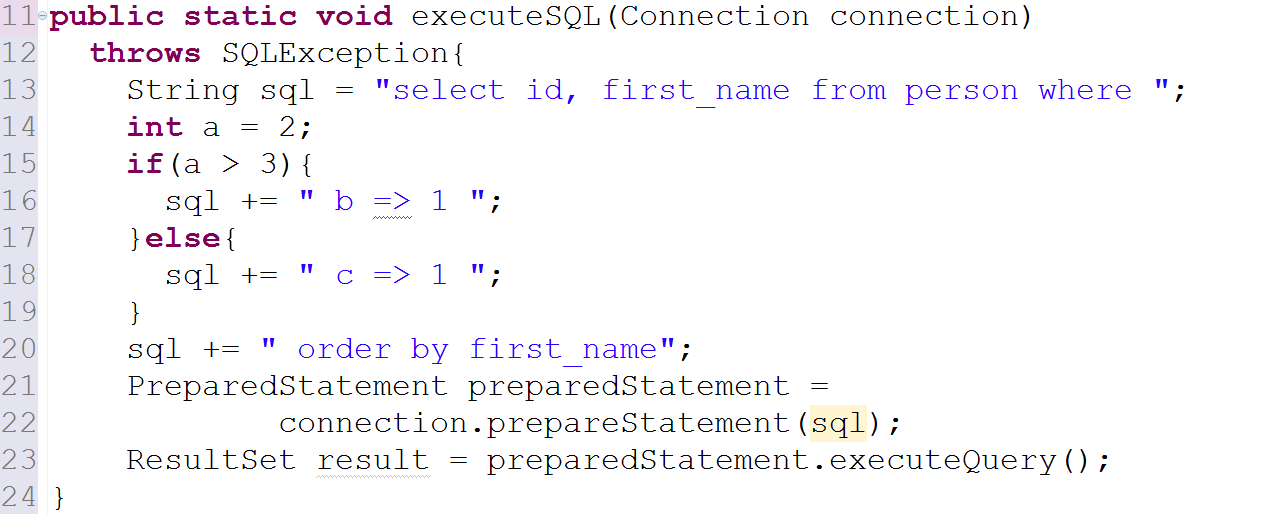
\includegraphics[scale=0.30]{Figures/Alvor.png}
    \end{center}
    \caption{Eclipse's text editor window with Alvor plugin}
    \label{alvor_pic}
\end{figure}

\subsection{IntelliLang}

IntelliLang\footnote{IntelliLang is a plugin offering a number of features related to the processing of embedded languages. Site: \url{https://www.jetbrains.com/idea/help/intellilang.html}} is a plugin for  IntelliJ IDEA\footnote{IntelliJ IDEA is an IDE for JVM-based development. Site: \url{http://www.jetbrains.com/idea/}} IDE that extends its functionality in the field of string-embedded languages support. Plugin can highlight embedded code, perform code completion and for some languages (JavaScript, XML) detect errors. IntelliLang does not perform strings with embedded code search: user should manually specify the strings to be analyzed. This makes it inconvenient to use the plugin for some tasks especially for reengineering. IntelliJ IDEA's text editor window is illustrated in Figure~\ref{IntelliLang_pic}. The method getHtml is marked by \verb|@Language("HTML")| attribute which means this method returns the string containing html code as a result. Despite the closing tag \verb|</body>| is missing in the 12 line, IntelliLang does not report the error as the plugin is not able to perform error checking for html language.

\begin{figure}[h!]
    \begin{center}
        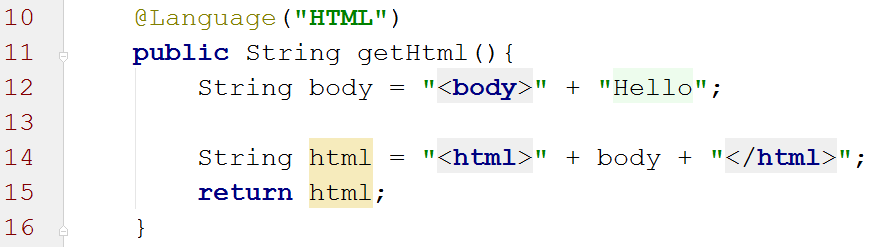
\includegraphics[scale=0.35]{Figures/IntelliLang.PNG}
    \end{center}
    \caption{IntelliJ IDEA's text editor window with IntelliLang plugin}
    \label{IntelliLang_pic}
\end{figure} 

\subsection{PhpStorm}

PhpStorm\footnote{IDE for PHP programming language. Site: \url{http://www.jetbrains.com/phpstorm/}} is an IDE for web-applications creating in PHP. PHP programs often contain embedded code in HTML, CSS, JavaScript, and SQL, and PhpStorm performs highlighting and code completion for it. However PhpStorm is not able to handle dynamically generated strings. Such an example can be seen in Figure~\ref{PHPStorm_pic}. The variable \verb|$string| contains html code, but it is not highlighted as its value is dynamically constructed. Moreover, PhpStorm does not report errors: even though the IDE highlighted the SQL code in the line 11, it did not indicate the error the query contains.

\begin{figure}[h!]
    \begin{center}
        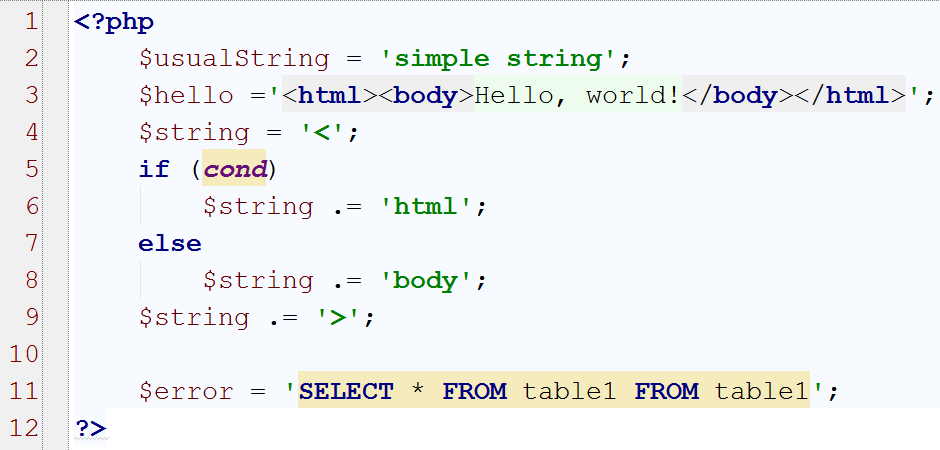
\includegraphics[scale=0.30]{Figures/PHPStorm.png}
    \end{center}
    \caption{PHPStorm's text editor window}
    \label{PHPStorm_pic}
\end{figure} 

\subsection{Varis}

Varis~\cite{Varis:ref} is a plugin for Eclipse that provides support of HTML, CSS, and JavaScript code embedded into PHP. The functionality includes code highlighting, completion, "jump to declaration", call graphs building for embedded JavaScript. Figure~\ref{varis_pic} illustrates code highlighting and completion functions. 

\begin{figure}[h!]
    \begin{center}
        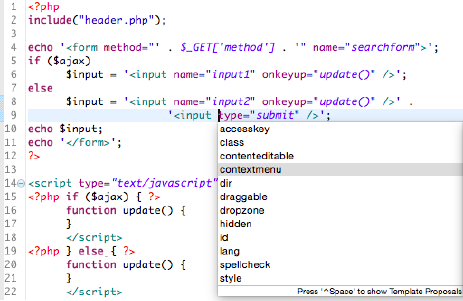
\includegraphics[scale=0.60]{Figures/Varis.PNG}
    \end{center}
    \caption{Eclipse's text editor window with Varis plugin}
    \label{varis_pic}
\end{figure} 

In conclusion one should note that along with specific drawbacks described tools either have limited functionality (JSA, PHPSA) which is difficult to extend, or support limited number of embedded languages (Alvor, PhpStorm and Varis). Furthermore, almost all the tools work with one specific host language.

\section{The platform}

Any language can be used both as string-embedded or host language. For each combination it could be necessary to solve different tasks: from errors detection to additional information extraction and metrics computation. As there are substantial number of languages combinations and different types of tasks, our research is not aiming to create a tool that handles all possible scenarios. The main goal is to create the platform that simplifies the process of building endpoint tools for the certain languages and tasks. The similar approach can be seen in the tools for compilers development. Usually such tools include lexical and syntax generators and utility functions libraries to simplify the process of  specific compiler creating.

Being complex and self-contained task, the host language analysis is assumed to be performed by some external tool. Moreover, this tool is assumed to return a source code's AST which contains the information needed for further steps as a result of it's work.

The platform is to perform the whole process of string-embedded languages handling. It includes the following steps:
\begin{itemize}
\item dynamically generated expressions can have a set of possible values so the approximation of the set is to be constructed;
\item lexical analysis is to be applied to the FSA that has been obtained after approximation;
\item syntax analysis is to be performed resulting in the parse forest;
\item parse forest analysis and semantics calculation is to be performed.
\end{itemize}

\subsection{Architecture}

The platform's architecture is shown in Figure~\ref{platform_architecture_ref}.

\begin{figure}[h!]
    \begin{center}
        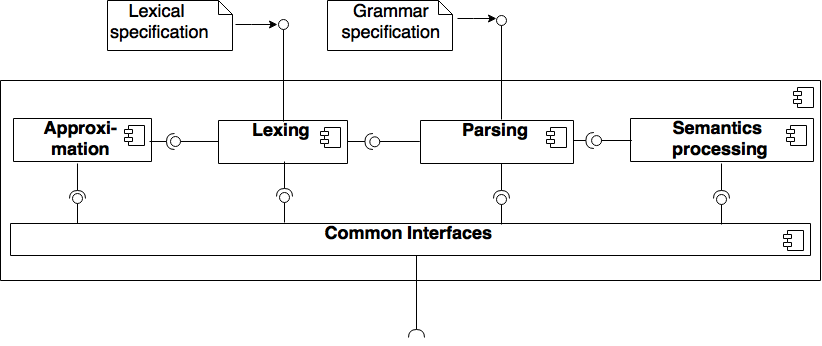
\includegraphics[scale=0.3]{Figures/SELYCcomponents.png}
    \end{center}
    \caption{The platform's architecture}
    \label{platform_architecture_ref}
\end{figure} 

The Approximation component is responsible for building the set of strings with embedded code that can be produced by the host language program. The elements of that set are to be statically analysed. This set can be considered as a language where the words are the strings with embedded code. In general the language can be recursively enumerable. Many problems are undecidable for this class of languages that makes it hard to work with. One possible solution is to build an upper regular approximation of the language we have. In other words we build the regular language that contains all the words of the language we have and, possibly, some other words. It is important to note that the regular language must be as close as possible to the language it approximates. It means the language must keep the number of "extra" words to a minimum. Despite the fact we end up with the approximation of the initial set, working with a regular language makes the further analysis much easier. Moreover, regular languages can always be represented as FSA that is convenient to manipulate.

The Approximation component accepts a generalized CFG with some additional information as an input. As an output it produces the FSA that encodes the approximated set of strings with embedded code.

The lexing component consist of two parts. The first one is the lexer's generator which generates finite-state transducer(FST,~~\cite{FST:ref}) from the provided lexical specification of the string-embedded-language. The second one is the interpreter which analyzes the data structure passed using generated FST. The lexing component accepts FSA over symbols alphabet and produces the FSA over alphabet of processed language tokens.

The parser generator is based on the RNGLR algorithm~\cite{RNGLR:ref}. Using the grammar of the language processed the generator builds parse tables. Then the analyzer, which is implemented as a separate library, parses the FSA that was obtained after the lexical analysis. The result is a shared packed parse forest (SPPF~\cite{SPPF:ref}) which is a compact structure that allows to reuse common nodes along different ASTs. This structure can be used for the further processing: for additional information extraction or to implement such IDE functionality as "go to definition".

\subsection{Approximation}

The process of building the set of strings with embedded code can be divided into two steps:
\begin{itemize}
\item finding the string expressions with embedded code in the source code;
\item building the set of possible values for found string expressions.
\end{itemize}

The first step is not implemented in our platform. This functionality is assumed to be implemented by the platform's user. The second step is performed by the platform and described in more detail below.

\subsubsection{Upper regular approximation building}

This section briefly describes the regular approximation building algorithm, presented in~\cite{Upper_Approximation:ref}. The paper~\cite{Upper_Approximation:ref} is devoted to the analysis of string expressions produced by PHP code. The analysis is aimed to find the expressions that can be used to perform malicious actions. We are interested in the algorithm presented because it guarantees building the upper approximation. Moreover, it handles most host language operations that can be used to form string expressions.

To begin with we introduce some definitions. \textit{Target expression} -- the string expression in the source code which possible values are to be built. \textit{Target node} -- the node in the control flow graph (CFG) containing target expression. \textit{Data-dependency graph (DDG)} -- directed graph that represents dependencies between instructions in the source code. Graph nodes correspond to expressions in the source code. The edge from the node \verb|X| to the node \verb|Y| indicates we need to calculate the expression in the node \verb|X| before we can calculate the expression in the node \verb|Y|.

As an example consider Listing ~\ref{code_fragment} where the reference to the \verb|"sql"| variable in the line 10 is chosen to be the target expression. Figure~\ref{flow_graph_pic} shows the CFG for the code fragment from the listing where the node 16 is a target node. DDG for the \verb|"sql"| reference is shown in Figure~\ref{data_dependency_pic}.

\begin{lstlisting}[label=code_fragment,caption=C\# code fragment]
Entries GetEntries(boolean cond) 
{
    string logMsg = "Selected";
    string sql = "SELECT * FROM ";
    if(cond)
      sql = sql + "Table1";
    else
      sql = sql + "Table2";
    Console.WriteLine(logMsg);
    return Db.Execute(sql);
}
\end{lstlisting}


\begin{figure}[h!]
    \begin{center}
        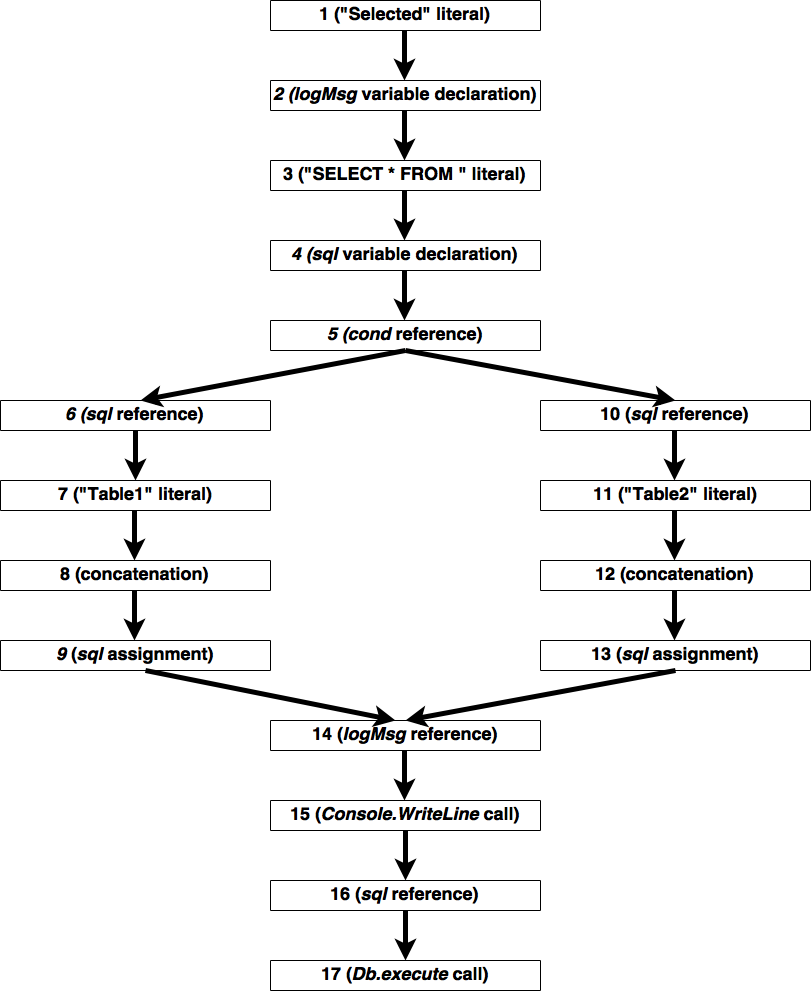
\includegraphics[scale=0.3]{Figures/Flow_graph.png}
    \end{center}
    \caption{Control flow graph for the code fragment from the Listing~\ref{code_fragment}}
    \label{flow_graph_pic}
\end{figure} 


\begin{figure}[h!]
    \begin{center}
        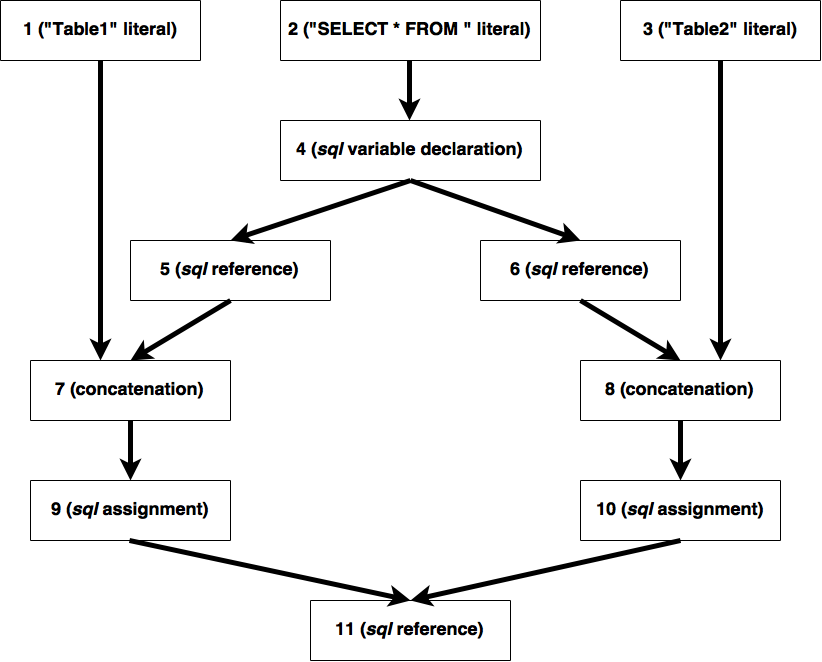
\includegraphics[scale=0.3]{Figures/Dependency_graph.png}
    \end{center}
    \caption{Data-dependency graph for the \texttt{"sql"} variable reference from the Listing~\ref{code_fragment}}
    \label{data_dependency_pic}
\end{figure} 

Further the following agreement about finite-state automata will be used. It is assumed every automaton has an additional state that is not shown explicitly. This state is called a sink state. The sink state is not a final one and transitions for all symbols of the automaton's alphabet lead to the sink state itself. When some automaton is mentioned in the text or illustrated in a picture transitions will be defined only for some symbols of the alphabet. It is assumed that if the transition for the symbol  \verb|'a'| from the state \verb|X| is not defined explicitly it leads to the sink state (see Figure~\ref{hi_pic}). Sink states are omitted for simplicity.

\begin{figure}[h!]
    \begin{center}
        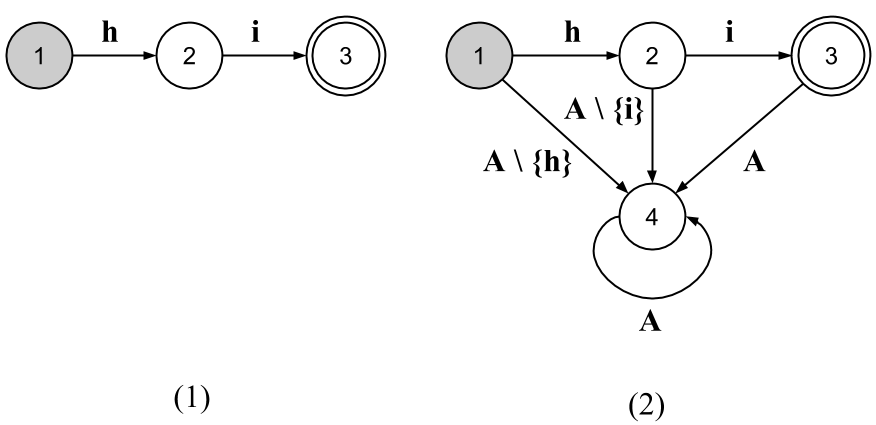
\includegraphics[scale=0.3]{Figures/automaton_with_sink.png}
    \end{center}
    \caption{Simplified illustration of the automaton over the alphabet A (1) and corresponding fully determined one with sink state (2)}
    \label{hi_pic}
\end{figure} 

Now we describe the regular approximation building algorithm presented in~\cite{Upper_Approximation:ref}. It consists of the following steps:
\begin{itemize}
\item control flow graph is created for the source code;
\item based on the CFG and some target node in it the data-dependency graph is computed;
\item finite state automata are constructed for the expressions in the DDG nodes. Automata are the upper approximations of the expressions' possible values sets. Automaton corresponding to the target node is returned as a result.
\end{itemize}

Let us see how exactly automata are built for the expressions in the nodes during the DDG traversal.

{\bf String literals.} The FSA for the string literal is an automaton that accepts only this literal. The example for the literal \verb|"hi"| is shown in Figure~\ref{hi_pic}.

\textbf{Strings concatenation.} The concatenation operation is performed on two automata that correspond to the operation arguments. Based on these automata the resulting one is built. It accepts the strings that consist of prefix and suffix. The prefix is any string accepted by the first argument automaton and the suffix is any word accepted by the second argument automaton (see Figure ~\ref{concat_pic}).

\begin{figure}[h!]
    \begin{center}
        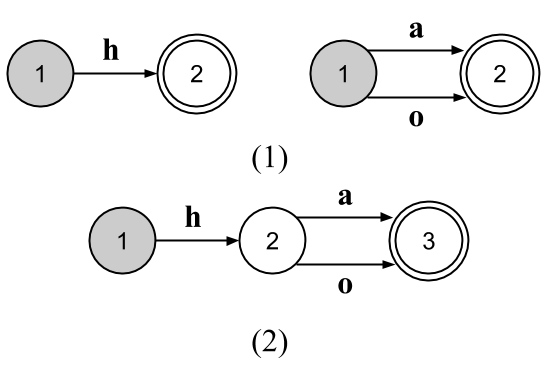
\includegraphics[scale=0.3]{Figures/automata_concat.png}
    \end{center}
    \caption{Argument automata (1) and their concatenation (2)}
    \label{concat_pic}
\end{figure} 

\textbf{Replace in strings.} Replace operation expects three automata as the arguments (see Figure~\ref{replace_pic}). The first one contains strings where the replace must be performed (Figure~\ref{replace_pic}(1)). The second one contains strings to be searched as substrings in the strings of the first automaton (Figure~\ref{replace_pic}(2)). The third one encodes the set of strings to be used as a replacement(Figure~\ref{replace_pic}(3)).

\begin{figure}[h!]
    \begin{center}
        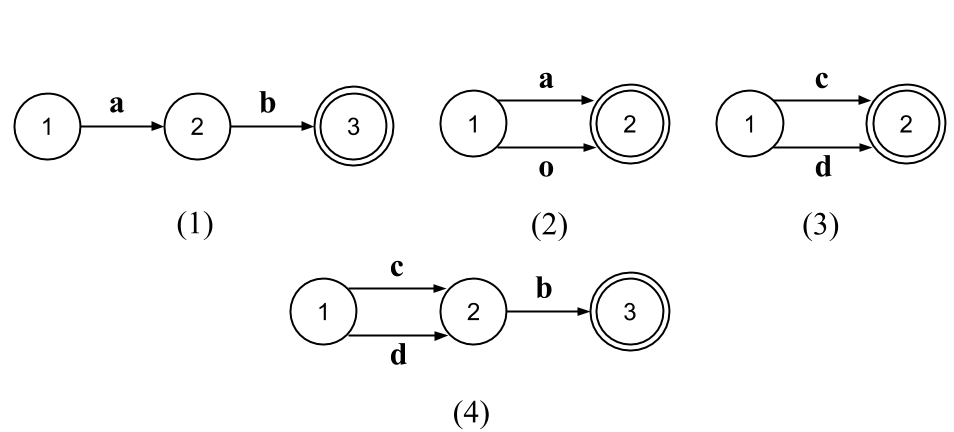
\includegraphics[scale=0.3]{Figures/automata_replace.png}
    \end{center}
    \caption{Replace operation arguments (1), (2) and (3) and the operation result (4)}
    \label{replace_pic}
\end{figure} 

\textbf{Conditional expressions (if, if-else).} Suppose there is node \verb|A| in the DDG. If the expression in the node \verb|A| depends on some expression that can be constructed in different branches of the conditional operator there are several (two in case of if-else) paths leading to the node \verb|A|. Same type expressions are constructed along all these paths. To collect the information about all these possible expressions one must union all the automata obtained after traversing each path leading to the node \verb|A|.

\textbf{Loops.} Loops processing is challenging. Firstly, during the static analysis it is often impossible to define how much iterations of the loop will be executed. So in general the loop produces an infinite language. Secondly, the language can be non regular and the example of such a case is shown on Listing~\ref{classic_example}. The fragment generates strings from the set $\{ a^nb^n |\; n = 1,\; 2 \ldots \}$, that is a classic example of a nonregular language.

\begin{lstlisting}[label=classic_example,caption=Loop with a replace operation in C\#]
String str = "ab";
for(...) {
  str = str.Replace ("ab", "aabb");
 }     	
Db.Execute(str);
\end{lstlisting}

To overcome the problems described the widening operator is used. The operator accepts two automata as the arguments and defines a special equivalence relation on the set of their states united. The equivalence classes formed by this equivalence relation are used as states for the resulting automaton, transitions are created based on the transitions of the argument automata. This resulting widened automaton accepts all the words accepted by the argument automata and generalizes these automata in some sense.

The operator is used for two automata that are the results of two successive loop iterations as follows:
$$
A_i' \;=\; \nabla (A_i \cup A_{i-1}, A_{i-1})
$$

where $A_i$, $A_{i-1}$ -- are the automata generated after current and previous iterations respectively, $\nabla$ -- widening operator. The $A_i'$ automaton is used as a new result of the current iteration. What is important is that the sequence $A'_i$, $i \;=\; 1, 2 \ldots$ is always converge~\cite{Upper_Approximation:ref}, i.e. beginning from some $m$:
$$
\forall i > m \colon A'_i \;=\; A'_{i+1} \;=\; R
$$

The notation  $A'_i \;=\; A'_{i+1}$ means the automata are equivalent, i.e. they define the same regular language. The automaton $R$ is set to be the result of the loop's approximation. In fact, here we solve the least fixed point computation problem.

Let us consider the example of widening operator usage for the loop in the Listing~\ref{example_loop}. The process of automata construction is presented in Figure~\ref{automata_loop_pic}. For each iteration the following automata are shown: the initial one -- constructed as a result of loop body processing; the united automaton -- constructed as a union operation result of the initial automaton and the automaton obtained in the previous iteration; the widened automaton -- constructed as a result of applying widening operator to the united automaton and  the automaton obtained in the previous iteration. If there is a dashed arrow from the automaton \verb|A| to automaton \verb|C| and from \verb|B| to \verb|C| the \verb|C| is constructed from \verb|A| and \verb|B| using the operation which name is written in the same line the automaton \verb|C| is placed (for example, union operation).

\begin{lstlisting}[label=example_loop,caption=Loop with concatenation on C\#]
String str = "a";
for(...) {
  str += "b";
}     	
Db.Execute(str);
\end{lstlisting}

It can be seen from the example the sequence of widened automata is converge on the third iteration. That is the widened automaton of the third iteration, accepting words from the set $\{ ab^{*} \}$, is set to be the approximation result of the loop from the Listing~\ref{example_loop}.

\begin{figure}[h!]
    \begin{center}
        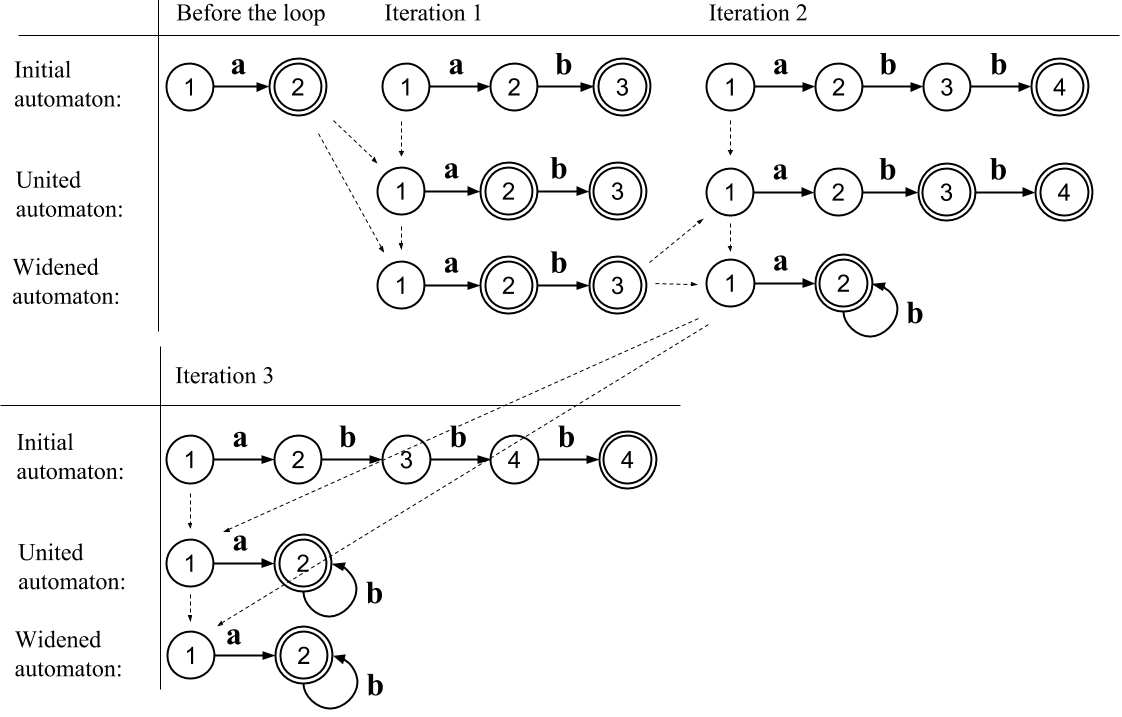
\includegraphics[scale=0.3]{Figures/automata_loop.png}
    \end{center}
    \caption{Approximation building for the loop from Listing~\ref{example_loop}}
    \label{automata_loop_pic}
\end{figure} 

\textbf{User input functions.} User input functions like reading from a console or file can return any strings and it is impossible to predict these strings values during the static analysis. Therefore, it is assumed the automaton for the return values of such functions is an automaton accepting any words.

Formal definitions of concatenation, replace and widening operations for the FSA are given in~\cite{Upper_Approximation:ref}.

Let us consider the example of FSA building for the DDG in Figure~\ref{data_dependency_pic}. The following steps will be performed.
\begin{enumerate}
\item Nodes 1, 2 and 3 contain literals, so for each of them the FSA accepting corresponding literal will be constructed.
\item After node 4 is processed the FSA constructed for node 2 will be bound to the name \verb|"sql"|.
\item For node 7 the automaton will be constructed which is the result of concatenation of the automaton named \verb|"sql"| and the automaton from node 1. The same is for node 8 but the second argument of the concatenation is obtained from node 3. The resulting automaton for node 7 will accept the literal  \texttt{"SELECT * FROM Table1"} and the automaton for node 8 -- literal \texttt{"SELECT * FROM Table2"}.
\item In nodes 9 and 10 the automata from nodes 7 and 8 respectively will be bound to name \verb|"sql"|.
\item The final node 11 is a node where alternative branches of conditional operator are merged. So the automata with the same names obtained from the alternative branches will be united here. That is, the resulting automaton for node 11 is the one that accepts both literals \texttt{"SELECT * FROM Table1"} and \texttt{"SELECT * FROM Table2"}.

\end{enumerate}

\subsubsection{Implementation details of the approximation algorithm}

One should note the implementation details of the described algorithm in our platform.

On the first step of the algorithm we create so called generalized CFG instead the usual one. The generalized CFG has the same structure as the usual one, but instructions in nodes are replaced with abstract ones. So in fact the generalized version represents the control flow of a pseudocode of the initial program. It is assumed that to build the approximation for some specific language one should convert language specific CFG to general one. This makes the platform able to support multiple host languages.

The approximation is built for some function (or method) where the strings with embedded code are constructed. During the processing of this function, the ones called from it are processed too. So the interprocedural approximation is built. To process the function calls the whole approximation algorithm is repeated recursively with the called function's return statement being a target expression. The recursion depth is constrained by some number that is defined as the algorithm's parameter and can be changed if needed. If the recursion depth becomes equal to the constraining parameter value the subsequent function calls are not processed anymore. The FSA accepting any words is used as the approximation result of this subsequent function calls.

The function called in source code under processing can be recursive itself. In this case the algorithm will always achieve constrained recursion depth and the approximation will be inaccurate because the FSA accepting any words will be used. In the case when called function is tail recursive we overcome described problem with special preprocessing. The generalized control flow subgraph  corresponding to tail recursive function call is replaced with the subgraph corresponding to the loop equivalent to this tail recursive function. This loop is processed then with widening operator as any other loop. For non tail recursive functions there is no special treatment for now.

\subsection{Lexical and syntax analysis}

The purpose of the lexical analysis is to extract tokens defined by the language specification from the input stream of symbols. Also the correspondence between lexical units and the source code must be preserved. The result of lexical analysis of the dynamically generated expression is a finite-state automaton over the alphabet of tokens. In the classic lexical analysis the token can be represented by some identifier and the subsequence of input symbols. In the case of dynamically generated expressions analysis the input symbols subsequence is replaced by the FSA representing the subset of all possible values of dynamically generated expression. Moreover, in the latter case for each symbol we must preserve the information about its position in the source code.

Lexical analysis consists of four steps. Firstly, the input FSA that was build by the approximator is transformed into the deterministic one. After that the FST is constructed based on the FSA. The next step is to build the composition of the obtained FST and the FST that was built based on the language specification. This second FST produces tokens as an output. The composition is a result of the consecutive application of these two transducers, i.e. an output of first FST is used as an input for the second. After that we obtain either a set of lexical errors or a FST with a pair on each edge. The first item in the pair is the symbol with the binding to the source code, the second one is a function that returns either token or nothing. If the previous step end up with no errors, the last step is an interpretation of the FST resulting in a finite-state automaton over the tokens alphabet.

This automaton is processed by the syntax analyzer. The analyzer is based on RNGLR~\cite{RNGLR:ref} algorithm which is a modification of Tomita's GLR-algorithm\cite{Tomita:ref}. Tomita's GLR algorithm allows to handle arbitrary context-free grammars. GLR handles Shift/Reduce and Reduce/Reduce conflicts -- situations when an available data are not enough to choose the correct way of parsing. Therefore, GLR processes all possible ways in case of conflict. So several derivation trees for a single input sequence can be obtained. The parser used in our platform extends this approach. The algorithm processes a token graph as an input. Herewith we meet a new situation when one node has several outgoing edges. We call this a "Shift/Shift" conflict despite the fact it is not an actual conflict because each way should be processed. More detail about the parser algorithm can be found in~\cite{AGLR:ref}. 

\subsection{SPPF analysis and semantics calculation}

The result of dynamically generated expressions parsing is a parse forest represented by the structure called SPPF~\cite{SPPF:ref}. This structure allows to reuse common subtrees for different trees.

Based on SPPF it is possible to build a so called compound control flow graph and try to solve classic static analysis tasks using it. When building compound CFG we assume that the string-embedded language grammar is a grammar of some programming language and that a mapping between non-terminals and CFG blocks is defined. For instance the \verb|"if_stmt"| non-terminal derivation should be treated as the conditional block in CFG. Other example is shown in Figure~\ref{simple_example_pic}, where the \verb|"assignment"| non-terminal derivation is treated as the assignment operation in CFG.

\begin{figure}[h!]
  \begin{center}
    \begin{subfigure}{0.3\textwidth}    
        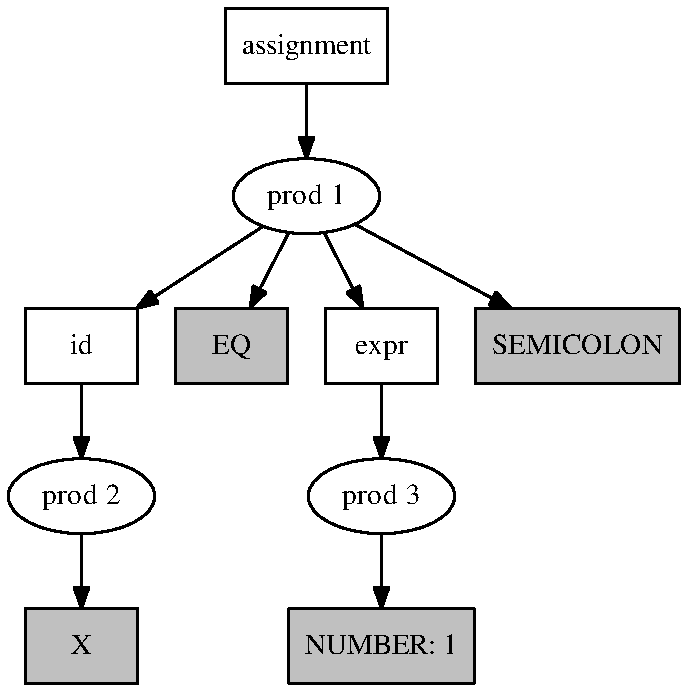
\includegraphics[scale=0.3]{Graphs/cfg_idea.pdf}    
    \caption{}
    \label{simple_a}
    \end{subfigure}
    \begin{subfigure}{0.1\textwidth}      
            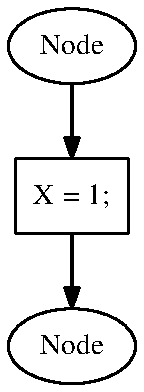
\includegraphics[scale=0.5]{Graphs/assignment_simple.pdf}        
     \caption{}
     \label{simple_b}
    \end{subfigure}
    \caption{\texttt{assignment} non-terminal derivation (\ref{simple_a}) and corresponding CFG block (\ref{simple_b})}
    \label{simple_example_pic}
  \end{center}
\end{figure}

Because of the fact that SPPF can contain several trees, the compound CFG can contain several usual CFGs. To make this possible an intermediate nodes are introduced. Further intermediate nodes will be called \textit{"nodes"} (in figures they will have oval shape) and CFG elements will be called \textit{"blocks"} (in the figures they will have rectangle shape). The derivation of \verb|"assignment"| non-terminal corresponding to sequences \verb|"X = 1;"| and \verb|"Y = 1;"| is shown in Figure~\ref{complicated_example_pic}. 

\begin{figure}[h!]
    \begin{center}
    \begin{subfigure}{0.3\textwidth}    
        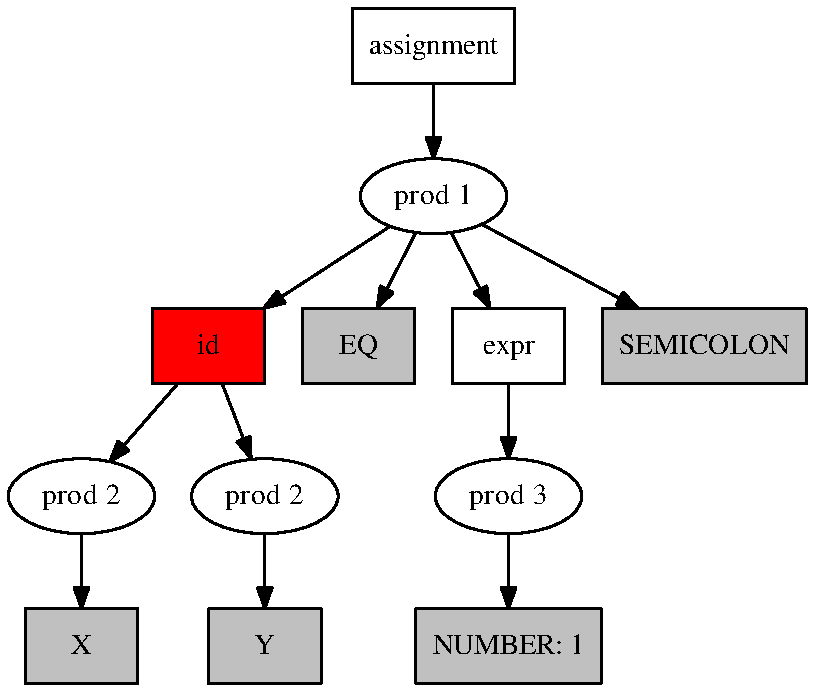
\includegraphics[scale=0.3]{Graphs/cfg_idea_complicated.pdf}    
    \caption{}
    \label{complicated_a}
    \end{subfigure}
    \begin{subfigure}{0.1\textwidth}      
            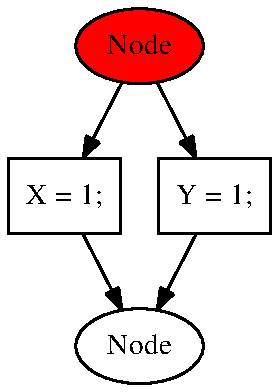
\includegraphics[scale=0.5]{Graphs/assignment_complicated.pdf}
        \caption{}
        \label{complicated_b}
    \end{subfigure}
    \caption{\texttt{"assignment"} non-terminal derivation (\ref{complicated_a}) and corresponding CFG blocks (\ref{complicated_b})}
    \label{complicated_example_pic}
    \end{center}
\end{figure}
Using obtained compound CFG one can solve the static analysis tasks. Consider definite assignment analysis as an example. Here we suppose that variable is defined in the statement $\alpha$ if and only if there is a variable definition along each of the evaluation paths from the program's start to the $\alpha$ statement. 

For each block $\alpha$ the following transitions are valid:
$$
before (\alpha) \;=\; \bigcap_{\beta \;\in\; pred(\alpha)} \;after(\beta)
$$
$$
after (\alpha) \;=\; before(\alpha) \cup gen(\alpha)
$$
where
\begin{itemize}
\item $before(\alpha)$ set contains variables defined before the statement $\alpha$;
\item $after(\alpha)$ set contains variables defined after the statement $\alpha$;
\item $gen(\alpha)$ set is empty if $\alpha$ is not an assignment block and contains left-hand operand of the assignment otherwise. 
\end{itemize}

As in case of usual CFG, the algorithm traverses the graph beginning from the start node for which the empty set is associated with. The only difference is that the $pred(\alpha)$ set contains nodes, not CFG blocks. But it is easy to define the required sets:
$$
before (\beta) \;=\; \bigcap_{\alpha \;\in\; pred(\beta)} \;after(\alpha)
$$
$$
after (\beta) \;=\; before (\beta)
$$
The compound CFG is shown in Figure~\ref{cfg_example}. In the red colored node only variable \verb|X| is defined. This node have two child blocks and the list containing variable \verb|X| is passed to each block. The \verb|"Y = X + 2;"| block adds the variable \verb|Y| to the list (because \verb|Y| is defined in this block), and the \verb|"Z = X * 3;"| block adds the variable \verb|Z|. These two blocks have the same child node, therefore the intersection of parents' lists is associated with it, i.e. the list containing the only variable \verb|X|. The list is passed when the block \verb|"X = Y * Z;"| is processed. Since passed list does not contain \verb|Y| and \verb|Z|, they will be reported as undefined variables.
\begin{figure}[h!]
    \begin{center}
        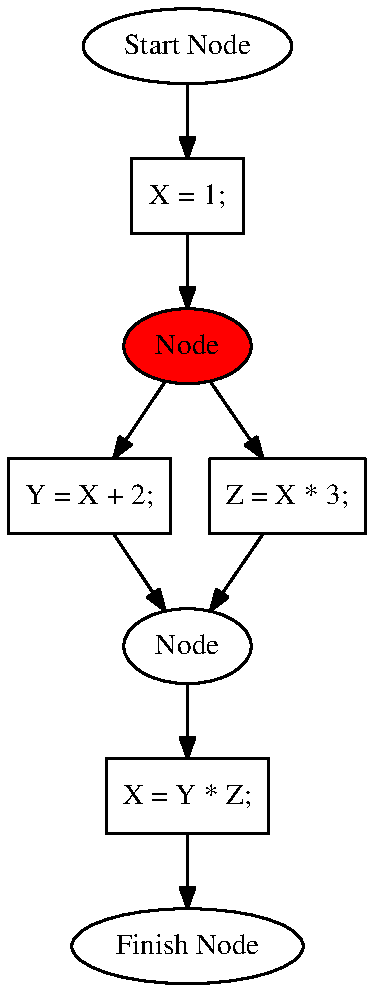
\includegraphics[scale=0.4]{Graphs/cfg_example.pdf}
    \end{center}
    \caption{Compound control flow graph}
    \label{cfg_example}
\end{figure} 

\section{Using the platform}

In order to use the platform a developer have to perform two steps.
\begin{itemize}
\item Add the host language support. To do this it is necessary to provide the module which for a source code on the host language can build a generalized CFG and mark target nodes in it. Generalized control flow graph specification is defined by the platform. The result of this module's work will be passed to the Approximation component as an input.
\item Add the support of the string-embedded language through the implementation of the common interface. To achieve this it is necessary to provide the lexical specification (needed for lexer generation) and the grammar (needed for parser generation) of the embedded language. After the lexer and parser are created developer can use the standard implementation of the interface functions.
\end{itemize}

After these steps are performed a developer obtains the tool which supports the desired string-embedded language inside the desired host one. An embedded code syntax highlighting, matching parentheses highlighting, and static errors detection becomes available for these pair of languages. Microsoft Visual Studio with the ReSharper\footnote{ReSharper is plugin to Microsoft Visual Studio, extending standard IDE functionality. Site: \url{http://www.jetbrains.com/resharper/}} plugin is used as a target IDE. The functionality currently available is not very rich, but the platform's architecture is designed for further extension.

Currently available functions can be configured by the user. Syntax highlighting can be configured by specifying the mapping between each token type and the color it should be highlighted with. Also user can choose which tokens are considered as paired: for each pair "left" and "right" elements are to be set (opening and closing parentheses, for instance). If a caret in the editor is located near one of the paired elements the other element corresponding to it will be highlighted.

\subsection{Evaluation}

To test the platform the tools for embedding T-SQL and arithmetic expressions language (called Calc) in C\# and JavaScript were implemented. The tools are designed to work on Microsoft .NET platform. The most popular IDE for the .NET platform is Microsoft Visual Studio. By default it has no string-embedded languages support. The implemented tools were integrated as extensions to ReSharper~--  a plugin to Microsoft Visual Studio, which extends the the default functionality of the IDE.

ReSharper has a freely available SDK containing most of the ReSharper's functionality, in particular the capability to build control flow graphs for the source code. The modules for building C\# and JavaScript specific CFGs and converting them to generalized ones were implemented using the SDK.

For strings with embedded code searching, an algorithm based on the special predefined set of functions (or methods) usage was implemented. These functions are called hotspots. What is special about these functions is that we know they expect a string with embedded code as an argument. In the source code we search calls of these hotspot functions and the arguments of the calls are set to be target expressions. The main idea of the approach is based on the fact, that the programs that construct the strings with embedded code often use some subsystem to execute it. The method \verb|"execute"| of the \verb|java.SQL.Statement| interface that is used in Java programs to execute SQL queries via JDBC technology can be considered as an example. In general the described approach does not always work correctly, but relative implementation simplicity is it's undoubted advantage.

The information about hotspots is stored in the configuration .xml file. For each hotspot it contains corresponding function's signature and the name of the embedded language the hotspot corresponds to. In the case of T-SQL a hotspot is a method or function named \verb|ExecuteImmediate|, in case of Calc -- named \verb|Eval|. It should be noted that hotspots for different embedded languages can occur in the same analyzed file with the source code.

Lexical and parser specifications were built for Calc and a subset of T-SQL languages. The lexer and parser were generated using these specifications. Xml files for syntax highlighting and set of classes for ReSharper integration were created during the parser generation.

\textbf{Syntax highlighting.} The example of T-SQL and Calc languages support in C\# is shown in Figure~\ref{highlighting}. Each language is highlighted separately: numbers in T-SQL query and in Calc expressions have different colors. Note the value of the \verb|"expr"| variable is formed in a loop using conditional statement and \textit{TrueCaseStr} function invocation. Plugin handles all these host language constructions for strings building so highlighting is performed even inside \textit{TrueCaseStr} method. 

\begin{figure}[h!]
    \begin{center}
        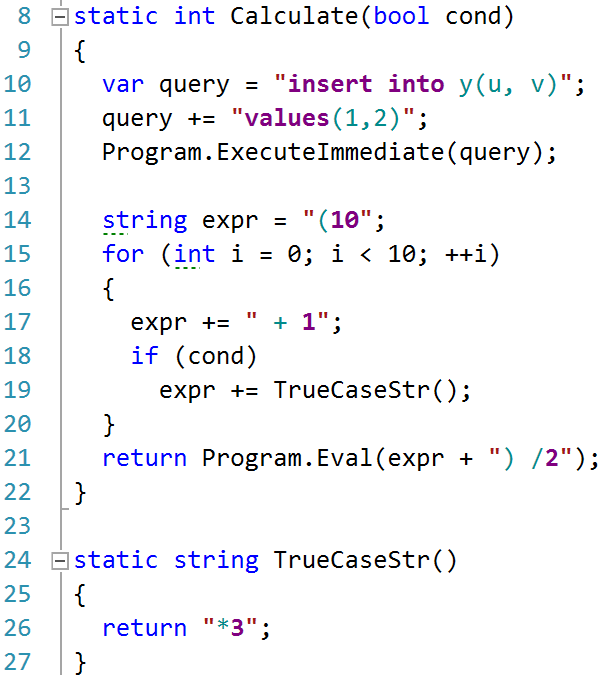
\includegraphics[scale=0.4]{Figures/sql_and_calc_cycle.PNG}
    \end{center}
    \caption{T-SQL and Calc syntax highlighting}
    \label{highlighting}
\end{figure}

\textbf{Static errors detection.} Plugin can find lexical errors and errors related to language semantics. In figure~\ref{static_error} \verb|"varY"| variable (line 22) is underlined as undefined because there exists the path that does not contain \verb|"varY"| declaration (if \verb|cond| parameter value is false).

\begin{figure}[h!]
    \begin{center}
        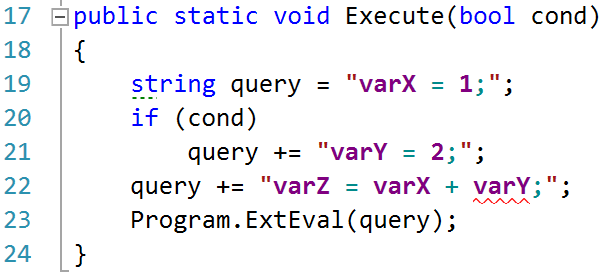
\includegraphics[scale=0.4]{Figures/Undefined_variable.PNG}
    \end{center}
    \caption{Static errors detection}
    \label{static_error}
\end{figure}

\textbf{Matching parenthesis highlighting.} Matching parenthesis highlighting improves the code readability. If a caret in the text editor is located near the one of paired symbols then the plugin should highlight it and it's matching symbol. The situation with dynamically generated expressions is different because one symbol in a pair may have several matching ones. Such a case is shown in Figure~\ref{brace1}. Opening brace (line 27) has two matching closing braces (lines 30 and 32) so three elements are highlighted. At the same time each closing brace has only one matching opening brace (Figure~\ref{brace2}).

\begin{figure}[h!]
  \begin{center}
    \begin{subfigure}[t]{0.2\textwidth}    
        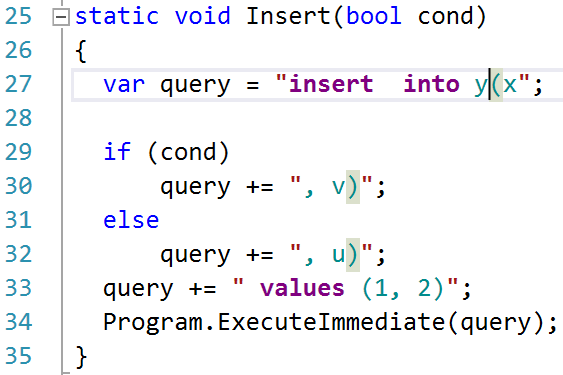
\includegraphics[scale=0.3]{Figures/brackets_one_to_many.PNG}    
    \caption{Multiple matches}
    \label{brace1}
    \end{subfigure}
	~\qquad
    \begin{subfigure}[t]{0.2\textwidth}      
            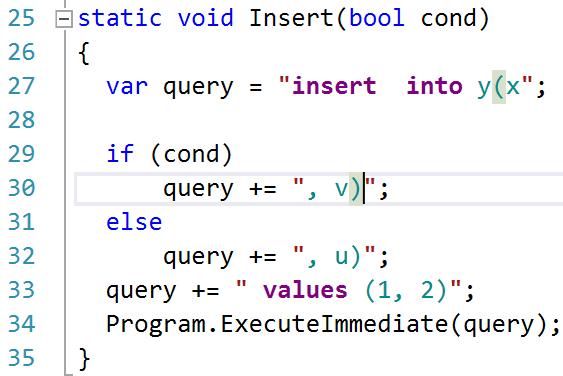
\includegraphics[scale=0.3]{Figures/brackets_one_to_one.PNG}        
        \caption{Single match}
        \label{brace2}
    \end{subfigure}
    \caption{Parenthesis highlighting}
    \label{braces}
  \end{center}
\end{figure}

\newpage
\section{Future work}

The future work will include the platform and plugin improvement. At the platform level the available functionality for embedded code processing will be extended. Particularly we plan to implement the mechanisms that will make string-embedded code transformations possible. Code transformations can be used to perform migration from one particular DBMS to another~\cite{Migration:ref} or to new embedding technology such as LINQ. This task is related to two problems: possibility of non-trivial transformations and proof of transformations correctness. Also we plan to implement type checking. For SQL it may be both a type checking inside the dynamically constructed queries and the consistency of the returned and expected types. In the later case we should check whether the type of the query result equals to the type of the variable in the host language the result is assigned to.

Performing semantic actions over SPPF is another important direction of the research. It is needed for refactoring, translation quality improvement, automation of the transition to a more reliable meta-programming tools.

\bibliographystyle{abbrv}
\bibliography{sigproc}

\balancecolumns

% \section{The {\secit Body} of The Paper}
% Typically, the body of a paper is organized
% into a hierarchical structure, with numbered or unnumbered
% headings for sections, subsections, sub-subsections, and even
% smaller sections.  The command \texttt{{\char'134}section} that
% precedes this paragraph is part of such a
% hierarchy.\footnote{This is the second footnote.  It
% starts a series of three footnotes that add nothing
% informational, but just give an idea of how footnotes work
% and look. It is a wordy one, just so you see
% how a longish one plays out.} \LaTeX\ handles the numbering
% and placement of these headings for you, when you use
% the appropriate heading commands around the titles
% of the headings.  If you want a sub-subsection or
% smaller part to be unnumbered in your output, simply append an
% asterisk to the command name.  Examples of both
% numbered and unnumbered headings will appear throughout the
% balance of this sample document.

% Because the entire article is contained in
% the \textbf{document} environment, you can indicate the
% start of a new paragraph with a blank line in your
% input file; that is why this sentence forms a separate paragraph.

% \subsection{Type Changes and {\subsecit Special} Characters}
% We have already seen several typeface changes in this sample.  You
% can indicate italicized words or phrases in your text with
% the command \texttt{{\char'134}textit}; emboldening with the
% command \texttt{{\char'134}textbf}
% and typewriter-style (for instance, for computer code) with
% \texttt{{\char'134}texttt}.  But remember, you do not
% have to indicate typestyle changes when such changes are
% part of the \textit{structural} elements of your
% article; for instance, the heading of this subsection will
% be in a sans serif\footnote{A third footnote, here.
% Let's make this a rather short one to
% see how it looks.} typeface, but that is handled by the
% document class file. Take care with the use
% of\footnote{A fourth, and last, footnote.}
% the curly braces in typeface changes; they mark
% the beginning and end of
% the text that is to be in the different typeface.

% You can use whatever symbols, accented characters, or
% non-English characters you need anywhere in your document;
% you can find a complete list of what is
% available in the \textit{\LaTeX\
% User's Guide}\cite{Lamport:LaTeX}.

% \subsection{Math Equations}
% You may want to display math equations in three distinct styles:
% inline, numbered or non-numbered display.  Each of
% the three are discussed in the next sections.

% \subsubsection{Inline (In-text) Equations}
% A formula that appears in the running text is called an
% inline or in-text formula.  It is produced by the
% \textbf{math} environment, which can be
% invoked with the usual \texttt{{\char'134}begin. . .{\char'134}end}
% construction or with the short form \texttt{\$. . .\$}. You
% can use any of the symbols and structures,
% from $\alpha$ to $\omega$, available in
% \LaTeX\cite{Lamport:LaTeX}; this section will simply show a
% few examples of in-text equations in context. Notice how
% this equation: \begin{math}\lim_{n\rightarrow \infty}x=0\end{math},
% set here in in-line math style, looks slightly different when
% set in display style.  (See next section).

% \subsubsection{Display Equations}
% A numbered display equation -- one set off by vertical space
% from the text and centered horizontally -- is produced
% by the \textbf{equation} environment. An unnumbered display
% equation is produced by the \textbf{displaymath} environment.

% Again, in either environment, you can use any of the symbols
% and structures available in \LaTeX; this section will just
% give a couple of examples of display equations in context.
% First, consider the equation, shown as an inline equation above:
% \begin{equation}\lim_{n\rightarrow \infty}x=0\end{equation}
% Notice how it is formatted somewhat differently in
% the \textbf{displaymath}
% environment.  Now, we'll enter an unnumbered equation:
% \begin{displaymath}\sum_{i=0}^{\infty} x + 1\end{displaymath}
% and follow it with another numbered equation:
% \begin{equation}\sum_{i=0}^{\infty}x_i=\int_{0}^{\pi+2} f\end{equation}
% just to demonstrate \LaTeX's able handling of numbering.

% \subsection{Citations}
% Citations to articles \cite{bowman:reasoning,
% clark:pct, braams:babel, herlihy:methodology},
% conference proceedings \cite{clark:pct} or
% books \cite{salas:calculus, Lamport:LaTeX} listed
% in the Bibliography section of your
% article will occur throughout the text of your article.
% You should use BibTeX to automatically produce this bibliography;
% you simply need to insert one of several citation commands with
% a key of the item cited in the proper location in
% the \texttt{.tex} file \cite{Lamport:LaTeX}.
% The key is a short reference you invent to uniquely
% identify each work; in this sample document, the key is
% the first author's surname and a
% word from the title.  This identifying key is included
% with each item in the \texttt{.bib} file for your article.

% The details of the construction of the \texttt{.bib} file
% are beyond the scope of this sample document, but more
% information can be found in the \textit{Author's Guide},
% and exhaustive details in the \textit{\LaTeX\ User's
% Guide}\cite{Lamport:LaTeX}.

% This article shows only the plainest form
% of the citation command, using \texttt{{\char'134}cite}.
% This is what is stipulated in the SIGS style specifications.
% No other citation format is endorsed or supported.

% \subsection{Tables}
% Because tables cannot be split across pages, the best
% placement for them is typically the top of the page
% nearest their initial cite.  To
% ensure this proper ``floating'' placement of tables, use the
% environment \textbf{table} to enclose the table's contents and
% the table caption.  The contents of the table itself must go
% in the \textbf{tabular} environment, to
% be aligned properly in rows and columns, with the desired
% horizontal and vertical rules.  Again, detailed instructions
% on \textbf{tabular} material
% is found in the \textit{\LaTeX\ User's Guide}.

% Immediately following this sentence is the point at which
% Table 1 is included in the input file; compare the
% placement of the table here with the table in the printed
% dvi output of this document.

% \begin{table}
% \centering
% \caption{Frequency of Special Characters}
% \begin{tabular}{|c|c|l|} \hline
% Non-English or Math&Frequency&Comments\\ \hline
% \O & 1 in 1,000& For Swedish names\\ \hline
% $\pi$ & 1 in 5& Common in math\\ \hline
% \$ & 4 in 5 & Used in business\\ \hline
% $\Psi^2_1$ & 1 in 40,000& Unexplained usage\\
% \hline\end{tabular}
% \end{table}

% To set a wider table, which takes up the whole width of
% the page's live area, use the environment
% \textbf{table*} to enclose the table's contents and
% the table caption.  As with a single-column table, this wide
% table will ``float" to a location deemed more desirable.
% Immediately following this sentence is the point at which
% Table 2 is included in the input file; again, it is
% instructive to compare the placement of the
% table here with the table in the printed dvi
% output of this document.


% \begin{table*}
% \centering
% \caption{Some Typical Commands}
% \begin{tabular}{|c|c|l|} \hline
% Command&A Number&Comments\\ \hline
% \texttt{{\char'134}alignauthor} & 100& Author alignment\\ \hline
% \texttt{{\char'134}numberofauthors}& 200& Author enumeration\\ \hline
% \texttt{{\char'134}table}& 300 & For tables\\ \hline
% \texttt{{\char'134}table*}& 400& For wider tables\\ \hline\end{tabular}
% \end{table*}
% % end the environment with {table*}, NOTE not {table}!

% \subsection{Figures}
% Like tables, figures cannot be split across pages; the
% best placement for them
% is typically the top or the bottom of the page nearest
% their initial cite.  To ensure this proper ``floating'' placement
% of figures, use the environment
% \textbf{figure} to enclose the figure and its caption.

% This sample document contains examples of \textbf{.pdf}
% and \textbf{.ps} files to be displayable with \LaTeX.  More
% details on each of these is found in the \textit{Author's Guide}.

% \begin{figure}
% \centering
% \epsfig{file=fly.pdf}
% \caption{A sample black and white graphic (.pdf format).}
% \end{figure}

% \begin{figure}
% \centering
% \epsfig{file=fly.pdf, height=1in, width=1in}
% \caption{A sample black and white graphic (.pdf format)
% that has been resized with the \texttt{epsfig} command.}
% \end{figure}


% As was the case with tables, you may want a figure
% that spans two columns.  To do this, and still to
% ensure proper ``floating'' placement of tables, use the environment

% \subsection{Theorem-like Constructs}
% Other common constructs that may occur in your article are
% the forms for logical constructs like theorems, axioms,
% corollaries and proofs.  There are
% two forms, one produced by the
% command \texttt{{\char'134}newtheorem} and the
% other by the command \texttt{{\char'134}newdef}; perhaps
% the clearest and easiest way to distinguish them is
% to compare the two in the output of this sample document:

% This uses the \textbf{theorem} environment, created by
% the\linebreak\texttt{{\char'134}newtheorem} command:
% \newtheorem{theorem}{Theorem}
% \begin{theorem}
% Let $f$ be continuous on $[a,b]$.  If $G$ is
% an antiderivative for $f$ on $[a,b]$, then
% \begin{displaymath}\int^b_af(t)dt = G(b) - G(a).\end{displaymath}
% \end{theorem}

% The other uses the \textbf{definition} environment, created
% by the \texttt{{\char'134}newdef} command:
% \newdef{definition}{Definition}
% \begin{definition}
% If $z$ is irrational, then by $e^z$ we mean the
% unique number which has
% logarithm $z$: \begin{displaymath}{\log e^z = z}\end{displaymath}
% \end{definition}

% Two lists of constructs that use one of these
% forms is given in the
% \textit{Author's  Guidelines}.

% There is one other similar construct environment, which is
% already set up
% for you; i.e. you must \textit{not} use
% a \texttt{{\char'134}newdef} command to
% create it: the \textbf{proof} environment.  Here
% is a example of its use:
% \begin{proof}
% Suppose on the contrary there exists a real number $L$ such that
% \begin{displaymath}
% \lim_{x\rightarrow\infty} \frac{f(x)}{g(x)} = L.
% \end{displaymath}
% Then
% \begin{displaymath}
% l=\lim_{x\rightarrow c} f(x)
% = \lim_{x\rightarrow c}
% \left[ g{x} \cdot \frac{f(x)}{g(x)} \right ]
% = \lim_{x\rightarrow c} g(x) \cdot \lim_{x\rightarrow c}
% \frac{f(x)}{g(x)} = 0\cdot L = 0,
% \end{displaymath}
% which contradicts our assumption that $l\neq 0$.
% \end{proof}

% Complete rules about using these environments and using the
% two different creation commands are in the
% \textit{Author's Guide}; please consult it for more
% detailed instructions.  If you need to use another construct,
% not listed therein, which you want to have the same
% formatting as the Theorem
% or the Definition\cite{salas:calculus} shown above,
% use the \texttt{{\char'134}newtheorem} or the
% \texttt{{\char'134}newdef} command,
% respectively, to create it.

% \subsection*{A {\secit Caveat} for the \TeX\ Expert}
% Because you have just been given permission to
% use the \texttt{{\char'134}newdef} command to create a
% new form, you might think you can
% use \TeX's \texttt{{\char'134}def} to create a
% new command: \textit{Please refrain from doing this!}
% Remember that your \LaTeX\ source code is primarily intended
% to create camera-ready copy, but may be converted
% to other forms -- e.g. HTML. If you inadvertently omit
% some or all of the \texttt{{\char'134}def}s recompilation will
% be, to say the least, problematic.

% \section{Conclusions}
% This paragraph will end the body of this sample document.
% Remember that you might still have Acknowledgments or
% Appendices; brief samples of these
% follow.  There is still the Bibliography to deal with; and
% we will make a disclaimer about that here: with the exception
% of the reference to the \LaTeX\ book, the citations in
% this paper are to articles which have nothing to
% do with the present subject and are used as
% examples only.
%\end{document}  % This is where a 'short' article might terminate

%ACKNOWLEDGMENTS are optional
% \section{Acknowledgments}
% This section is optional; it is a location for you
% to acknowledge grants, funding, editing assistance and
% what have you.  In the present case, for example, the
% authors would like to thank Gerald Murray of ACM for
% his help in codifying this \textit{Author's Guide}
% and the \textbf{.cls} and \textbf{.tex} files that it describes.

%
% The following two commands are all you need in the
% initial runs of your .tex file to
% produce the bibliography for the citations in your paper.
% \bibliographystyle{abbrv}
% \bibliography{sigproc}  % sigproc.bib is the name of the Bibliography in this case
% You must have a proper ".bib" file
%  and remember to run:
% latex bibtex latex latex
% to resolve all references
%
% ACM needs 'a single self-contained file'!
%
%APPENDICES are optional
%\balancecolumns
% \appendix
%Appendix A
% \section{Headings in Appendices}
% The rules about hierarchical headings discussed above for
% the body of the article are different in the appendices.
% In the \textbf{appendix} environment, the command
% \textbf{section} is used to
% indicate the start of each Appendix, with alphabetic order
% designation (i.e. the first is A, the second B, etc.) and
% a title (if you include one).  So, if you need
% hierarchical structure
% \textit{within} an Appendix, start with \textbf{subsection} as the
% highest level. Here is an outline of the body of this
% document in Appendix-appropriate form:
% \subsection{Introduction}
% \subsection{The Body of the Paper}
% \subsubsection{Type Changes and  Special Characters}
% \subsubsection{Math Equations}
% \paragraph{Inline (In-text) Equations}
% \paragraph{Display Equations}
% \subsubsection{Citations}
% \subsubsection{Tables}
% \subsubsection{Figures}
% \subsubsection{Theorem-like Constructs}
% \subsubsection*{A Caveat for the \TeX\ Expert}
% \subsection{Conclusions}
% \subsection{Acknowledgments}
% \subsection{Additional Authors}
% This section is inserted by \LaTeX; you do not insert it.
% You just add the names and information in the
% \texttt{{\char'134}additionalauthors} command at the start
% of the document.
% \subsection{References}
% Generated by bibtex from your ~.bib file.  Run latex,
% then bibtex, then latex twice (to resolve references)
% to create the ~.bbl file.  Insert that ~.bbl file into
% the .tex source file and comment out
% the command \texttt{{\char'134}thebibliography}.
% This next section command marks the start of
% Appendix B, and does not continue the present hierarchy
% \section{More Help for the Hardy}
% The sig-alternate.cls file itself is chock-full of succinct
% and helpful comments.  If you consider yourself a moderately
% experienced to expert user of \LaTeX, you may find reading
% it useful but please remember not to change it.
%\balancecolumns % GM June 2007
% That's all folks!
\end{document}